\documentclass{article}

\usepackage{natbib}

% for equation*
\usepackage{amsmath}

% for scalebox,...
\usepackage{graphics}

% for automated hyperlinks on sections and \ref's:
% - hide hyperref links with white pdfborder (this is more portable than the hidelinks option)
\usepackage[pdfborder={0 0 0}]{hyperref}

% for comment environment:
\usepackage{verbatim}

% for pseudocode
\usepackage{algorithm}
\usepackage[noend]{algpseudocode}

% Defining this variable turns on extra sections which should be useful from a development
% perspective, but would not typically be included in a theoretical methods description.
% Comment/remove this line to render a more concise methods summary.
\let\IncludeDevelopmentDetail


% GLOBALLY change all typewriter fonts to enable hyphenation:
\DeclareFontFamily{\encodingdefault}{\ttdefault}{\hyphenchar\font=`\-}

%---------------------------------------------------------------------
% Custom commands and environments:
%

% 'raggedParagraph' is an environment to enable raggedright for a single paragraph
%
% This is used for all "Implementation details" sections so that code symbols entered
% with the verbatim command, such as "\verb|FooClass::foo_method|" will not spill into
% the right margin.
%
\newenvironment{raggedParagraph}[1]
{
\begin{paragraph} {#1}
\raggedright
}
{
\end{paragraph}
}

% simple scientific notation:
\newcommand{\e}[1]{\ensuremath{\times 10^{#1}}}


%---------------------------------------------------------------------

\title{Methods for Manta Structural Variant and Indel Caller}


\begin{document}

\maketitle

\tableofcontents

\section{Purpose}

On any release branch, the methods described here should reflect the default implementation in the source repository containing this document.

\section{Manta Workflow Overview}

Manta's structural variant calling workflow contains two major phases. In the first phase, the genome is scanned to build a genome-wide breakend graph. In the second phase, edges of this graph are analyzed to generate SV candidates, each of which is assembled, scored according to diploid or somatic quality models and reported. A high-level schematic of the workflow is described in Figure \ref{fig:workflow} below.

\begin{figure}[h]
\centerline{
  \scalebox{1.2}{
    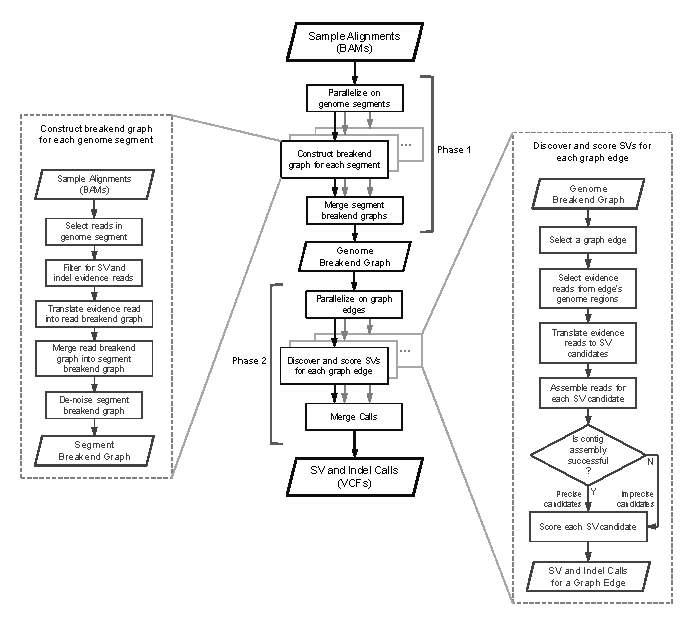
\includegraphics{figures/workflow.eps}
  }
}
\caption{High-level processing steps and parallelization strategy in Manta's variant calling workflow.}
\label{fig:workflow}
\end{figure}

For the breakend graph created in phase one, each node represents a region of the genome where evidence for at least one breakend exists. Edges represent evidence of a junction between two breakends. By design, the edges in the breakend graph do not correspond to a specific SV candidate hypotheses, instead they represent evidence of potentially many junctions between regions. This lack of specificity allows the graph for all variant types in the genome to be compactly represented in a small memory footprint.

Phase two of Manta's workflow occurs after the complete breakend graph is created. Given the complete breakend graph, sets of graph edges are approximated as independent structural variant discovery problems and each of these sets is analyzed in parallel. Each structural variant discovery process starts from one (or more) edges from the breakend graph, discovers any structural variant candidates on its edge (or edges) and executes assembly, scoring and reporting for each candidate variant.

Manta's two phase structure enables a high level of parallelization. In the first phase a set of independent tasks generate subsets of the breakend graph corresponding to small segments of the genome (Manta's default segment size is 12 Megabases). At the end of this phase there is a final step to merge all genome segment graphs into a single graph for the whole genome. In the next phase the genome breakend graph edges are divided among a set of independent SV discovery processes. The output of all such discovery processes are merged to produce the final set of SV candidates and calls.

\section{Fragment size and depth statistics}

Before entering the first major phase of the workflow, Manta completes a rapid estimation of fragment size and read depth information. During this step the sequence fragment size distribution is estimated for each BAM file provided as input. To accomplish this efficiently, the size distribution is sampled so that only a small subset of the input sequence alignments for each sample need to be scanned. To reduce regional bias, this step cycles through several small sections from different chromosomes, each containing 100k innie read pairs, until the size distribution convergences. Reads are filtered from this process to reduce bias from fragments associated with SVs or small indels, this filtration includes removing any reads marked as secondary, supplemental, filtered or PCR duplicates. Both reads from a pair must be mapped to the same chromosome with a non-zero mapping quality, align without indels and must not include a split-read annotation (i.e. using the BAM ``SA" tag). After filtration, a read is loaded in a small buffer of size 1000, where the the ratio of abnormal innie reads (i.e. those with a fragment size larger than 5000) is checked. If the abnorma-read ratio is higher than 1\%, the buffered reads are discarded, and reads are continually sampled from the next section that is 1\% of the chromosome length away from the current position.

A related prerequisite step Manta performs is estimation of the sequencing depth for each chromosome. For somatic analysis this depth is only computed for the normal sample. This information is used downstream to filter out high-depth regions (details below) when Manta is run in its default whole genome sequencing mode, these values can be ignored for exome or other targeted analyses.

\subsection{Chromosome depth estimation}

For each chromosome, depth is estimated using a modified median calculation. As a first step, each chromosome is partitioned into segments of similar size to ensure the estimation process samples several chromosome regions. The chromosome is divided into the smallest number of segments no larger than $S_{max}$, where all segments have nearly equal size (all sizes must be $S$ or $S+1$, given smallest segment size of $S$). If this procedure results in more than 20 segments, then $S_{max}$ is doubled until 20 or fewer segments are found. $S_{max}$ is initialized to 2 Mbase.

The depth estimation procedure repeatedly cycles through all segments. Within each segment, at least 40,000 reads are scanned before moving to the next segment (additional reads are scanned until the mapping position changes.) After the target number of reads have been scanned from every segment in the chromosome, the procedure returns to the first position and repeats this procedure starting from the last unscanned position. The process repeats until the all reads in all segments are scanned or the depth estimate converges.

Each scanned read is removed from consideration if it is marked as filtered, PCR duplicate, secondary, supplemental, or if the read is unmapped. Otherwise the read alignment is ignored and the read is applied to a simple depth pileup assuming a complete and ungapped alignment starting from the mapping position. Every 1M reads triggers a convergence check, but only after every chromosome segment has been sampled at least once.

Depth is estimated from the resulting pileup, using a simple median over all depth observations from the pileup structure excluding zero counts. Convergence is checked between the depth estimate of the last convergence check and the current one. An absolute change of less than 0.05 is treated as converged (or given the median case, the integer median estimates must be an exact match).

The depth estimation procedure is run separately for each non-tumor sample, and all high-depth thresholds are set based on the sum of depth estimates over these samples.

\section{Manta Workflow Phase One: Breakend graph construction}

\subsection{Breakend graph structure}

The breakend graph $G$ describes regions of the genome which are connected by one or more possible breakend junctions. The graph, $G = (V, E)$, comprises a set of nodes $V$ and a set of directed edges $E$. Each node $v \in V$ is annotated with a contiguous genome segment containing one or more breakends. Each edge $e \in E$ connects nodes where evidence of a breakend junction exists. Edge direction is set from the node where a direct read mapping observation is observed to the node where the read mapping is inferred. Self-edges indicate that there is evidence for one or more breakend junctions within the region defined by the node incident to the self-edge. Typically this indicates that a small indel could exist in the region. Each edge is annotated with an evidence weight, which enumerates all of the individual paired and split-read observations supporting the edge. Supporting observations are weighted by reliability, for instance, the weight of an anomalous read pair insert size observation is reduced as the implied fragment length of the pair approaches non-anomalous values. To facilitate recovery of read evidence associated with each graph node in downstream hypothesis generation steps, each node is also annotated with a region spanning the mapping location for all the node's read evidence.

This graph is designed to contain only the information required to partition the SV discovery problem into a set of independent SV discovery processes in the second workflow phase. It does not provide sufficient detail to support candidate discovery on its own. According to this design the breakend graph for full human genomes can be represented in a small memory footprint. In practice, a case has yet to be found where the graph (and its indexing structures) require greater than 2Gb, including breakend graphs for high-depth FFPE tumor/normal pairs.

\subsection{Genome segment distribution}

The breakend graph is constructed by first computing subgraphs corresponding to individual segments of the genome. Graph construction is run in parallel over a set of disjoint segments covering the entire genome, followed by a graph merging step. Given a maximum segment size (default is 12 Mb), each chromosome is partitioned into a set of nearly equal size segments without exceeding the maximum segment size, and one subgraph construction process is started for each.

\subsection{Genome segment breakend graph construction}

For each genome segment, input BAM file(s) are scanned over the corresponding genome region for breakend associated reads, which are merged into the segment's breakend graph. To do so, each mapped read in the genome segment must first pass through a filtration process to eliminate noise. Any remaining reads are then translated into a set of small breakend graphs (currently each of these graphs is a single edge connecting either one or two nodes). These graphs are merged into the segment's breakend graph, where threshold-based merging and de-noising procedures are implemented to prune edges which do not have sufficient evidence. The de-noising procedure is constrained from running on an edge until both regions connected by the edge have been scanned for evidence. The details of this procedure are as follows.

\subsubsection{Filtration}
For graph construction, reads are removed if they are marked as secondary, filtered or PCR duplicates. Reads also must be mapped and have a mapping quality of 15 or greater. A read pair is determined to be anomalous if it has (1) unexpected read orientation, (2) a mate mapping to another chromosome, or (3) an unexpectedly large fragment size. For the fragment size to be considered anomalous at the initial filtration stage, it must be greater than $1.5s_{max}$, where $s_{max}$ is the 99th percentile of the sample fragment size distribution. If the read pair is not found to be anomalous, the read is additionally checked for (1) indels of at least the minimum candidate indel size (default: 8), (2) a split-read annotated using the BAM record's ``SA" tag, or (3) an alignment where 5 contiguous matches to the reference cannot be found within 7 bases from either end of the read. If none of these read alignment conditions exist and the read pair is not anomalous, the read pair is filtered out of the graph construction process.

\subsubsection{Read pair translation to breakend graph set}
\label{sec:pair2graph}

Each unfiltered read pair is translated into a set of breakend graphs via a two step process. The read pair is first translated to a set of SV candidates. The translation process allows for the possibility that the BAM record for only one read of the pair is available, in which case the length and alignment of the remote mate read is approximated. The logic to translate read pairs to SV candidates is the same as that used in SV hypothesis generation during Manta's second phase.

The translation of each read (or read pair) into a set of SV candidates proceeds as follows:
\begin{itemize}
\item \textit{Anomalous Read Pairs} We create an SV candidate for any read pair with an unexpected orientation, chimeric mapping or anomalously large fragment size. To determine large fragment size we find $r_p$, the extent of the read pair in reference coordinates, and accept a read pair if $r_p > s_{max} + c_{min}$, where $c_{min}$ is the minimum candidate indel size. If accepted, the candidate breakend regions extend from the end of each read to length $\max(40, s_{br} - r_1 - r_2)$, where $r_1$ and $r_2$ provide the extent of read 1 and read 2 alignments in reference coordinates, and $s_{br}  = f_l s_{lr} + (1 - f_l) s_{sr}$, where $s_{lr}$ and $s_{sr}$ are the 90th and 75th percentile of the fragment size distribution respectively. The $f_l$ term is defined such that shorter candidate breakend regions are used for smaller candidate deletions, as described below

\begin{equation*}
f_l =
\left\{
\begin{array}{cl}
1 & \mbox{ chimeric/anomalous orientation,} \\
0 & \mbox{ $r_p < s_{sr}$, } \\
1 & \mbox{ $r_p > s_{lr}$, } \\
\frac{r_p - s_{sr}} {s_{lr} - s_{sr}} & \mbox{otherwise.}
\end{array}
\right.
\end{equation*}

\item \textit{Read alignment gaps} Any gaps indicated in the an individual read alignment are translated into SV candidates if the total inserted or deleted sequence length exceeds the minimum indel candidate size. The SV candidate breakend regions are expanded by 20 bases in each direction form the exact breakpoint implied in the read alignment.

\item \textit{Poorly aligned read edges} For each read edge we force any soft-clipped regions to align to the reference and then evaluate for a high density of base mismatches at the read edge. To do so we find $d_{m}$, the minimum distance from the edge where the next 5 positions match the reference. If $d_{m}$ is at least 8 and at least 3/4 of the basecalls in the range [1,$d_{m}$] have quality 20 or greater, we define a complex region candidate, which has one region extending 20 bases in each direction from the interior edge of the poorly-aligned read end.

Complex region candidates indicate that there is evidence for small indels or SVs within a region without proposing a specific SV hypothesis. Assembly of the complex region will be performed to refine the candidate into a specific set of indels.

\item \textit{Split-reads} Split-read alignments as indicated using the BAM record ``SA" tag convention will generate SV candidates as well. For reads which are split into no more than 2 segments, where both segments have a mapping quality of at least 15, the SV candidate implied by the split-read junction is generated. The two SV candidate regions are extended by 20 bases in each direction from the implied junction site.

\end{itemize}

These SV candidates are translated into breakend graph elements by converting SV breakend regions into graph nodes spanning the same region and representing the connection between regions as a directed edge from the region of direct evidence (the locally observed read of a pair), to the region of indirect evidence (the remote read of a pair). Complex region candidates are translated into a single graph node spanning the candidate region with a self-edge added to indicate that there is evidence for novel breakend junctions within the candidate region. Each edge has an `evidence weight' of 3, except for edges corresponding to read pairs which imply a fragment size close to the anomalous size threshold (less than $4s_{max}$), which are given an evidence weight of 1.

\subsubsection{Merge and de-noising procedure}

In the procedure above, each SV-associated read or read pair is translated into one or more single-edge breakend graphs. Each one of the these single-edge breakend graphs is then sequentially merged into the breakend graph for the entire genomic segment. Merging is performed using a procedure which is general to any two breakend graphs. The high-level steps to this procedure are (1) take the union of the two input graphs, (2) find nodes from the graph union which qualify for merging, and (3) merge qualifying sets of nodes.

The node merging criteria are described in more detail below, the underlying rationale for this merging process is that each graph node represents a region of the genome and therefore two graph nodes representing sufficiently similar regions of the genome could be regarded as `matching' nodes representing the same region. Similarly two edges connecting two sets of matching nodes could be regarded as `matching' edges sharing an SV evidence association between the same two regions. Note that this concept of sharing SV evidence between similar regions of the genome is distinct from the concept of identifying shared evidence for the same SV, the purpose of the breakend graph is only to cluster SV evidence between similar regions, it is expected that each edge of the merged breakend graph could potentially contain evidence for multiple distinct SVs.

\renewcommand{\algorithmicrequire}{\textbf{Input:}}
\renewcommand{\algorithmicensure}{\textbf{Output:}}
\newcommand*\Let[2]{\State #1 $\gets$ #2}


\begin{algorithm}[h]
\floatname{algorithm}{Method}
\caption{Merge breakend graphs}
\label{method:merge}
\begin{algorithmic}[1]
\Require{Two breakend graphs $G_1$ and $G_2$}
\Ensure{Merged breakend graph $G$}

\Procedure{MergeGraphs}{$G_1,G_2$}
\State $G \gets G_1 \cup G_2$
\State \Call{AnnotateMergeableNodes}{$G$}
\State \Call{MergeNodes}{$G$}
\EndProcedure
\end{algorithmic}
\end{algorithm}

The high level merge procedure is outlined in Method \ref{method:merge}.The two input graphs are merged by taking their union, identifying and annotating nodes in the graph union which are eligible for merging (described in Method \ref{method:annotate}), and executing the eligible node merges (described in Method \ref{method:mergenodes}).

\begin{algorithm}[t!]
\floatname{algorithm}{Method}
\caption{Annotate mergeable graph nodes}
\label{method:annotate}
\begin{algorithmic}[1]
\Require{Breakend graph $G$}
\Ensure{Breakend graph $G$ with annotation of mergeable nodes}
\Procedure{AnnotateMergeableNodes}{$G$}
\For {node $v$ in $G$} \label{lst:line:clear}
\State mergeable[$v$] $\gets$ false
\EndFor
\For {node $v$ in $G$}  \label{lst:line:sigstart}
\For {node $w$ in adjacent[$v$]}
\If {evidence[$(v,w)$] $\geq e_s$}
\State mergeable[$v$] $\gets$ true
\State mergeable[$w$] $\gets$ true   \label{lst:line:sigend}
\EndIf
\EndFor
\EndFor
\For {node $v$ in $G$} \label{lst:line:noisestart}
\For {node $w$ in adjacent[$v$]}
\State $M \gets \{v,w\}$
\State $e_{\text{merged}} \gets $ evidence[$(v,w)$]
\For {node $x$ in \Call{IntersectingNodes}{$G$,$w$}}
\For {node $y$ in adjacent[$x$]}
\If {$y \in $ \Call{IntersectingNodes}{$G$,$v$}}
\State $e_{\text{merged}} \gets e_{\text{merged}} +$ evidence[$(x,y)$]
\State $M \gets M \cup \{x,y\}$
\EndIf
\EndFor
\EndFor
\If {$e_{\text{merged}} \geq e_s$}
\For {node $m$ in $M$}
\State mergeable[$m$] $\gets$ true \label{lst:line:noiseend}
\EndFor
\EndIf
\EndFor
\EndFor
\EndProcedure
\Statex

\Procedure{IntersectingNodes}{$G$,$v$}
\State $W \gets \{\}$
\For {node $w$ in $G$, $w \neq v$}
\If {region[$v$] $\cap$ region[$w$]}
\State $W \gets W \cup \{w\}$
\EndIf
\EndFor
\State \Return $W$
\EndProcedure

\end{algorithmic}
\end{algorithm}


The procedure used to identify `mergeable' nodes in a breakend graph is shown in Method \ref{method:annotate}. The first major step (lines \ref{lst:line:sigstart}-\ref{lst:line:sigend}) is to find all nodes incident on an edge with evidence weight already meeting the signal threshold $e_s$. These nodes are annotated as eligible for merging. The second step of the annotation procedure (lines \ref{lst:line:noisestart}-\ref{lst:line:noiseend}) is to find all sets of nodes which, if merged, would result in merged nodes incident on edges with an evidence weight of at least $e_s$. This is accomplished as follows: for each edge in the graph, $(v,w)$, all `intersecting' edges $(x,y)$ are found, where the genomic regions annotated for nodes $v$ and $x$ intersect, as do the regions for nodes $w$ and $y$. If the total evidence weight of the starting edge and all intersecting edges ($e_{\text{merged}}$ in Method \ref{method:annotate}) meets the signal threshold $e_s$, then all nodes incident on these edges ($M$) are made eligible for merging in the next step of the merge procedure.


\begin{algorithm}[t!]
\floatname{algorithm}{Method}
\caption{Merge all graph nodes annotated as mergeable}
\label{method:mergenodes}
\begin{algorithmic}[1]
\Require{Breakend graph $G$ with annotation of mergeable nodes}
\Ensure{Breakend graph $G$ with eligible nodes merged}
\Procedure{MergeNodes}{$G$}
\State $R \gets \{\}$
\For {node $v$ in $G$, mergeable[$v$] is true} \label{lst:line:findstart}
\Loop
\State $W \gets$ \Call{IntersectingNodes}{$G$,$v$}
\If {$W = \{\}$} break \EndIf
\For {node $w$ in $W$, mergeable[$w$] is true} \label{lst:line:findend}
\State region[$v$] $\gets$ region[$v$] $\cup$ region[$w$] \label{lst:line:regionstart}
\State region[$w$] $\gets \{\}$ \label{lst:line:regionend}
\For {node $x$ in adjacent[$w$]}
\State \Call{MergeEdgeEvidence}{$v$,$w$,$x$}
\EndFor
\State $R \gets R \cup \{w\}$
\EndFor
\EndLoop
\EndFor
\State $G \gets G \setminus R$
\EndProcedure
\Statex

\Procedure{IntersectingNodes}{$G$,$v$}
\State $W \gets \{\}$
\For {node $w$ in $G$, $w \neq v$}
\If {region[$v$] $\cap$ region[$w$]}
\State $W \gets W \cup \{w\}$
\EndIf
\EndFor
\State \Return $W$
\EndProcedure
\Statex

\Procedure{MergeEdgeEvidence}{$v$,$w$,$x$} \label{lst:line:mee}
\If    {$w = x$}
\State evidence[$(v,v)$] $\gets$ evidence[$(v,v)$] + evidence[$(w,w)$]
\ElsIf {$v = x$}
\State $e_{\text{max}} \gets$ max(evidence[$(w,v)$],evidence[$(v,w)$])
\State evidence[$(v,v)$] $\gets$ evidence[$(v,v)$] + $e_{\text{max}}$
\Else
\State evidence[$(v,x)$] $\gets$ evidence[$(v,x)$] + evidence[$(w,x)$]
\State evidence[$(x,v)$] $\gets$ evidence[$(x,v)$] + evidence[$(x,w)$]
\EndIf
\EndProcedure
\end{algorithmic}
\end{algorithm}

Following annotation of nodes for merge eligibility, the procedure to execute merging for eligible nodes is applied as described in Method \ref{method:mergenodes}. For two nodes to merge, both must be annotated as eligible and their genomic region annotation must intersect. In Method \ref{method:mergenodes}, lines \ref{lst:line:findstart}-\ref{lst:line:findend} describe the procedure to produce such qualifying node pairs $v$ and $w$. To merge node $w$ into $v$, first the union of the region annotation from both nodes is applied to $v$, and the region of $w$ is cleared (lines \ref{lst:line:regionstart}-\ref{lst:line:regionend}). Next the evidence weight of all edges incident on $w$ are transferred to the merged node $v$ as described in MergeEdgeEvidence (line \ref{lst:line:mee}) for any node $x$ adjacent to $w$. For each merged node pair, the non-merged node, $w$, is accumulated in $R$ so that these nodes can be removed from the merged graph as the final step of the procedure.

In practice, the evidence weight signal threshold $e_s$ defaults to 9 and the evidence weight applied for an non-penalized split or paired read observation (as described in the previous section) is 3. Thus the above described breakend graph merging procedure effectively requires 3 split or paired read observations supporting the same region association before merging this evidence in the breakend graph.

% TODO The graph complexity filtration procedure in the paragraph below seems to have been left in an inaccurate state for some time and should be rewritten from the implementation. A TDR ticket (MANTA-1355) has been created for this update.
% Specific problems are:
% 1. There is no reference to the 'locus' concept from source code
% 2. The abort is actually applied to a whole locus instead of just the candidate merge node.
% 3. The complexity check has now been turned off for loci containing more than two nodes.
The breakend graph merge procedure can be limited under conditions of high graph complexity. If the search for all nodes intersecting a candidate merge node (as described in the IntersectingNodes procedure in Method \ref{method:annotate}) results in 500 or more nodes or greater than 0.5 nodes per base in the search region, the merge of the associated candidate edge is stopped. This step is designed to limit graph complexity in repetitive and pericentromeric regions.

As the target genome segment is scanned, the region breakend graph is periodically de-noised. The procedure is only performed for edges where the input alignment files have been scanned over the genomic regions of the nodes incident on the edge (excluding small buffer zones at the edges of the scanned genome segments). For any edge $e = (v,w)$ which is eligible for de-noising, if both evidence[$(v,w)$] and evidence[$(w,v)$] are less than $e_s$, the edge is removed from the graph, together with any nodes isolated by the edge removal.

\subsection{Global breakend graph construction}

Using the graph merging and de-noising procedures described in the previous section, it is straightforward to create the global breakend graph from the set of genome segment graphs. To do so the genome segment breakend graphs are sequentially merged into the global breakend graph using the breakend graph merge procedure described in the previous section. This merging step is followed by a final de-noising step which is the same as that described for genome segments above, except that all edges are treated as eligible for de-noising.

\section{Manta Workflow Phase Two: Hypothesis generation and scoring}

After construction of the global breakend graph, each set of independent breakend-associations is distributed among a group of SV discovery workers running in parallel. Each worker handles SV hypothesis generation, scoring and reporting for its input breakend associations. At present an independent breakend association is approximated as a single breakend graph edge, however Manta's design enables larger highly-connected subgraphs to be distributed to SV discovery workers in the future to directly generate larger multi-junction SV hypotheses.

\subsection{SV hypothesis generation}

Hypothesis generation currently proceeds from a single breakend graph edge. The noise filtration criteria for hypothesis generation are more strict than that used in the graph de-noising step, so that any edge $e = (v,w)$ where either evidence[$(v,w)$] or evidence[$(w,v)$] is less than $e_s$ is filtered.

For any non-filtered edge, the first step of hypothesis generation is to find all reads potentially associated with SVs which span the node(s) connected by the input graph edge. For this purpose, reads are searched over the evidence range recorded for each graph node. The evidence range is a superset of the node's breakend-associated range describing the region containing mapped reads which contribute breakend evidence for the node. These regions are scanned for read evidence using the same read filtration criteria described for graph generation in the first phase of the workflow.

After gathering SV-associated reads from the targeted regions, each read or read pair is translated into a set of SV candidates using the same logic described for graph construction above. Any SV candidate which does not intersect the targeted graph edge is discarded. Intersecting the graph edge is defined as having one breakend intersect each of the two genomic regions connected by the edge. The SV candidates remaining after this filtration process are merged into a combined SV candidate set -- any two SV candidates are merged if both of their breakend regions intersect and the expected breakend orientation for each region matches. Complex region candidates targeting small indels are only merged with other complex region candidates. It is expected that this merging procedure could be improved with additional steps to reduce over-clustering by determining if the hypothesis region supports more than one breakend and splitting the candidate appropriately. Thus far, the simple intersection-based hypothesis generation described above has not been implicated as a significant source of errors compared to other workflow components.

\subsubsection{Building multi-junction SV candidates}

Standard SV candidates (ie. non-complex candidates) represent a single novel junction between two genomic regions. At a larger scale, it is helpful to group together multiple junctions which have proximal in-phase breakends, with these grouped junctions being reported and/or scored as a single event. An example of such an event is a reciprocal translocation, which is composed of two junctions.

Manta has limited support for multi-junction event detection and scoring. This process begins after the initial SV hypothesis generation step by grouping junctions into candidate multi-junction events. This process currently only considers standard (non-complex) SV candidates. Non-inversion intrachromosomal events of size 100000 or less are also excluded from multi-junction event detection to reduce spurious associations. Given this filtered set of input SV candidates, the method searches for pairs of junctions where the two junctions (1) have breakends oriented in opposite directions at both junction ends
(2) have breakends with genomic regions centered within 1000 bases of each other at both junction ends (3) must have been discovered from the analysis of the same breakend graph edge. If more than one partner junction is eligible for grouping with a given junction, the pair with the lowest breakend region distance is selected -- such that only 2 junctions can be grouped together.

The multi-junction candidate search is currently limited to grouping together no more than 2 junctions for simplicity, in principle the method could be expanded to look for transitive associations over a larger set of junctions. To do this, constraint (3) above would need to be relaxed by ensuring that all edges possibly participating in the multi-junction event are analyzed by the same process (at present edges are distributed to independent processes for analysis).

\subsubsection{Early SV candidate filtration}

Before proceeding to downstream refinement steps, filters are applied to the standard and complex SV candidates. Standard SV filters are as follows:

\begin{enumerate}
    \item Standard SV candidates are filtered out if they are supported only by \textit{semi-mapped} anomalous read pairs. A \textit{semi-mapped} read pair refers to pairs where one read has a mapping quality of zero.
    \item Standard SV candidates are filtered out if they have fewer than 3 supporting spanning observations. A multi-junction SV candidate will fail this filter only if all individual junctions fail the filter.
    \item Standard SV candidates are filtered if the frequency of spanning read evidence is insufficient to reject (at $\alpha = 0.03$) a null model based on the \textit{spanning evidence noise rate} according to a one-sided binomial exact test. The estimation of \textit{spanning evidence noise rate} is described below. This test result is ignored if an SV candidate is grouped into a multi-junction event. This filter is skipped for RNA-Seq analysis. Note that this filter is intended to conservatively reject only very unlikely candidates, and is an important part of controlling total runtime in noisy samples (such as FFPE), where high background chimera rates could otherwise create very large numbers of spurious SV candidates.
\end{enumerate}

Filters for complex SVs are:

\begin{enumerate}
    \item Complex SV candidates are filtered out if they have fewer than 2 supporting observations of the same type associated with evidence of an indel (e.g. soft-clipping, etc).
    \item Complex SV candidates are filtered if the frequency of assembly evidence is insufficient to reject (at $\alpha = 0.005$) a null model based on the \textit{assembly evidence noise rate} according to a one-sided binomial exact test. The definition of assembly evidence and estimation procedure for \textit{assembly evidence noise rate} are described below.
\end{enumerate}

\paragraph{Noise Rates estimated from input read alignments}

The \textit{spanning evidence noise rate} and \textit{assembly evidence noise rate} used in the above filtration process are based on read counts accumulated during the first phase of Manta's workflow.

The \textit{spanning evidence noise rate} is based on the number of spanning (anomalous read pairs and split reads)  observations $s$ vs all reads observed $n$. Including pseudocounts, the estimate for this rate is $(s + 10) / (n + 1000)$.

\textit{Assembly evidence} observations are reads with poorly aligned edges (either soft-clipped or having a high mismatch density) as described above in section ``\nameref{sec:pair2graph}''. The \textit{assembly evidence noise rate} is based on the count of assembly evidence, $p$ vs all reads observed $n$. Including pseudocounts, the estimate for this rate is $(p + 10) / (n + 1000)$.

Given multiple alignment files, the above noise rates will be estimated independently for each alignment file, but only the maximum estimated noise rate will be kept for the purpose of SV candidate significance testing.



\subsection{SV hypothesis refinement}

Initial SV hypothesis generation translates each graph edge into a set of low-resolution SV candidates, where breakends are associated with an imprecise region. In the refinement step, each low-resolution SV candidate is translated into a set of basepair-resolution SV candidates via local read assembly. If the assembly procedure fails to produce at least one basepair-resolution candidate, then the low-resolution candidate can still be scored and reported in the variant caller output as an imprecise variant. If assembly fails for a complex region candidate associated with small indels, the candidate is discarded.

Hypothesis refinement is described below in two alternate forms: standard SV assembly describes the case of two remote breakend regions associated with a specific SV candidate; complex region assembly describes the case of a single breakend region where small indels or SVs are likely to exist, but no specific variant hypothesis exists.


\subsubsection{Contig assembly}

The contig assembly procedure gathers SV-associated reads from the candidate region or regions and assembles these reads into contigs intended to represent variant haplotypes.

As a first step, expanded breakend regions are defined, which will be scanned for assembly evidence and used for aligning any assembled contigs back to the reference. These regions are an expansion of the breakend regions of the low-resolution input SV candidate. Regions are expanded by 250 bases for conventional SV candidates and 700 bases for complex region candidates.

Candidate assembly reads are gathered from all expanded breakend regions. The input reads are assembled without considering their reverse complement sequences, because their orientation in the alternate contig can be inferred from either the mapped portion of the read or a mapped mate pair. In cases where the orientation of the two breakends is not the same (such as for an inversion), input read orientation is standardized to be consistent with the first breakend. Reads are selected as input to the assembly process by similar criteria to those used for hypothesis generation, but specific to the expected breakend direction and otherwise somewhat more permissive than the criteria used elsewhere. Relaxed filtration criteria include: no minimum mapping quality level, reads with poorly aligned read edge segments are accepted at length 4 (compared to length 8 elsewhere in the workflow), and unmapped reads which have a mapped partner in the target region are included. To improve the assembly of mobile element insertions, mate reads are recovered for chimeric read pairs when the local read of a chimeric read pair (found in the target assembly region) has a mapping quality of at least 15 and the remote read of the pair has a mapping quality of 0. This search for chimeric mate reads is disabled when Manta is run for tumor/normal subtraction due to high spurious chimera rates in FFPE tumor samples.

The selected reads are assembled using a simple algorithm implicitly based on the popular de Bruijn graph approach originated by Pevzner \citep{pevzner2001}. We note here that the orientation of each unmapped assembly read is determined by the orientation of its mapped partner, avoiding the need to deduce this during the assembly. Assembly is attempted over a series of word sizes, starting from a minimum value which is increased until repeat filtration criteria are met or the maximum word size is reached. The method currently uses a minimum word size of 41 and maximum size 76, the word size is incremented by 5.

For a given word size $k$, a word list is made of all $k$-mers present in the input reads. A seed list, as a subset of the word list, is also made by excluding the $k$-mers that form a cycle of size less than 50 in the graph. The most frequent $k$-mer in the seed list, given it has the most supporting reads, is selected as a seed for the resulting contig assembly. The contig is extended from that seed in each direction by choosing $k$-mers from the word list having a $k-1$ overlap with the contig end. To avoid haplotype switching, reads that support the contig are tracked at each extension point. When there are multiple potential extensions, a $k$-mer is selected so that the current extension has the highest consistency of supporting reads with the previous extensions. The extension ends when there is no overlapping $k$-mer from a previous supporting read, or when the selected $k$-mer has already occurred in the contig (i.e. being repetitive). The contig is then collected, and each $k$-mer used to contruct the contig is removed from the seed list if contained. The contig construction procedure is repeated to generate multiple contigs until all seeds in the list are exhausted. If any of the returned contigs ends at a repetitive $k$-mer, the word size is incremented by one step, and the contig assembly procedure is restarted. All the contigs generated with the previous word size is considered as psuedo reads to roll in the next iteration of contig assembly, similar to the assembly method described in \cite{tigra2014}.

Finally, a greedy procedure is applied to select the constructed contigs in the order of the number of effective supporting reads and contig length. An effective supporting read cannot be a psuedo read, nor support any contigs that have been selected previously. The selection process is repeated until there is no more contig available with the minimum number of effective supporting reads (defaults to 1), or the maximum number of assembled contigs (defaults to 10) is met.

\subsubsection{Contig alignment for large SVs} For large SV candidates spanning two distinct regions of the genome, the reference sequences are extracted from the two expected breakend regions, and the order and/or orientation of the references is adjusted such that if the candidate SV exists, the left-most segment of the SV contig should align to the first transformed reference region and the right-most contig segment should align to the second reference region. The contig is aligned across the two reference regions using a variant of Smith-Waterman-Gotoh alignment (\cite{smith1981,gotoh1982}) where a `jump' state is included which can only be entered from the match state for the first reference segment and only exits to the match or insert states of the second reference segment. The state transitions of this alignment scheme are shown in Figure \ref{fig:jumpstate}.

\begin{figure}[!tpb]
\centerline{
  \scalebox{0.48}{
    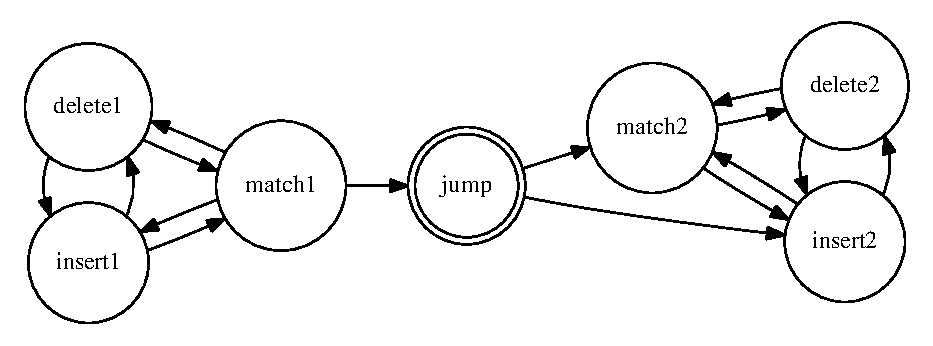
\includegraphics{figures/jumpstate.eps}
  }
}
\caption{State transitions for Manta's structural variant contig aligner. The alignment scheme uses conventional Smith-Waterman-Gotoh style affine gap alignment for the reference region in the vicinity of each breakend (possibly after strand reversal), with an additional `jump' state which provides a transition between the two breakend alignment regions. Note that a direct transition from the jump state to an insertion is allowed to enable alignment of novel sequence insertions at the breakend junction. In this case the insertion invokes standard affine gap penalties. Self-edges are not shown for clarity.}
\label{fig:jumpstate}
\end{figure}

The alignment scores used for each reference segment are (2,-8,-12,-1) for match, mismatch, gap open and gap extend. Switching between insertion and deletion states is allowed at no cost. Scores to transition into and extend the 'jump' state are -100 and 0, respectively. The jump state is entered from any point in reference segment 1 and exits to any point in reference segment 2. The alignments resulting from this method are only used when a transition through the jump state occurs. In addition, each of the two alignment segments flanking the jump state are required to extend at least 30 bases with an alignment score no less than 75\% of the perfect match score for the flanking alignment segment. If more than one contig meets all quality criteria, the contig with the highest alignment score is selected. When a contig and alignment meet all quality criteria, the reference orientation and ordering transformations applied before alignment are reversed to express the refined basepair-resolution structural variant candidate in standard reference genome coordinates.


\subsubsection{Contig alignment for complex region candidates}
Complex regions are segments of the genome targeted for assembly without a specific variant hypothesis. For this reason the problem of aligning contigs for these regions is somewhat more difficult than for specific large SV candidates, because a wide range of variant sizes are possible. This is reflected in the indel aligner that handles both small and large indels.

The indel aligner is a variant on a standard affine-gap scheme, in which a second pair of delete and insert states are added for large indels. Alignment scores for standard alignment states are (2, -8, -24, -1) for match, mismatch, gap open, and gap extend. Open and extend scores for 'large' gaps are -100 and 0. Transitions are allowed between standard insertions and deletions but disallowed between the large indel states.

All indels larger than the minimum indel size are identified by the indel aligner. For each indel, the flanking alignment quality criteria described above for large SVs is also applied to filter out noise alignments. To further reduce false positive calls in repetitive regions, an additional filter is applied to complex region candidates: the left and right segments of the contig flanking a candidate indel are checked for uniqueness in the local reference context. Contig alignments are filtered out if either of the two flanking contig segments can be aligned equally well to multiple locations within 500bp of the target reference region. Among contigs meeting all quality criteria, the ones with 'large' gaps are prioritized during contig selection. If there are more than one contig with 'large' gaps, or if all contigs have no 'large' gap, the contig with the highest alignment score is selected.

\subsubsection{Large Insertions}

Fully assembled large insertions will be detected by the standard contig assembly and alignment pipeline described above. Additional logic is added to detect and report the signature of a large insertion represented by two contig alignments which are consistent with left and right breakends of a large insertion. Under this scheme, all contig alignments are checked for the a signature of a high quality alignment for only a left or right subsegment of the contig. If two contigs form a left and right alignment pair implying two breakends within 35 bases then an imprecise long insertion is reported. In this case the left and right sides of the insert sequence are reported for an insertion of unknown total size.

\subsubsection{Post-alignment}
Following alignment of either complex region or standard SV candidates, the homology length and inserted sequence at the breakend junction are extracted from the alignment so that these can be included in the candidate scoring and reporting stages.

\paragraph{Late SV candidate filtration}

Candidates are filtered following SV hypothesis refinement as follows:

\begin{enumerate}
    \item Standard SV candidates are filtered out if they have fewer than 3 supporting spanning observations.
    \item Multi-junction SV candidates are filtered if every SV candidate junction in the candidate has fewer than 3 supporting spanning observations; each individual junction is filtered if it has fewer than 2 supporting spanning observations.
    \item Any complex SV candidates which failed to assemble are filtered.
    \item SV candidates below the minimum candidate SV size (8 by default) are filtered.
\end{enumerate}

\ifx\IncludeDevelopmentDetail

\begin{raggedParagraph}{Implementation details}

All late sv filtration logic is implemented in \verb|checkJunctionsToFilter|.

\end{raggedParagraph}

\fi % IncludeDevelopmentDetail

\paragraph{Candidate output}

Following the late filtration steps, the total set of refined candidates (or imprecise candidates in the case of assembly failure) are reported to a `candidate' VCF file. This file does not include scoring or quality filtration information but may be useful in a number of contexts, such as: (1) applications which are not supported by Manta's current scoring models (2) as a method development aid (3) as input to a small variant caller or another SV scoring/genotyping method.

\subsection{Scoring}

Following initial SV hypothesis generation, refinement via assembly, and filtration, all candidate variants are scored. In this phase, multiple scoring models can be applied to the candidate variants. Manta currently applies a diploid scoring model for one or more diploid samples (treated as unrelated), as well as a somatic scoring model when a tumor and matched normal sample pair are given.

\subsubsection{Diploid scoring model}

The diploid scoring model produces diploid genotype probabilities for each candidate structural variant. Most candidates are approximated as independent for scoring purposes, therefore we apply a simple model with a single alternate allele, that is, for reference and alternate alleles $A = \{r,x\}$ the genotype states at each allele are restricted to $G = \{rr, rx, xx\}$. We solve for the posterior probability over G using

\begin{equation*}
P( G \vert D ) \propto P( D \vert G )  P (G)
\end{equation*}

\noindent
where $D$ are all supporting read fragments for either allele. The prior $P(G)$ is

\newcommand{\thz}{\theta_{\textnormal{SV}}}

\begin{equation*}
P ( G ) =
\left\{
\begin{array}{rl}
\thz      & \mbox{ if $rx$} \\
\thz / 2  & \mbox{ if $xx$} \\
1 - \thz 3 / 2  & \mbox{ if $rr$}
\end{array}
\right.
\end{equation*}

\noindent
where the SV heterozygosity is $\thz = 1\e{-5}$.

The likelihood $P(D \vert G)$ is computed assuming that each read fragment $d \in D$ represents an independent observation of the sample

\begin{equation*}
P(D \vert G) = \prod_{d \in D} P(d \vert G)
\end{equation*}

\noindent
where the fragment likelihood is

\begin{equation*}
P(d \vert G) = \sum_{a \in A} P(d \vert a) P(a|G)
\end{equation*}

This likelihood for each fragment to support a given allele $P(d \vert a)$ is common to both diploid and somatic scoring models, and is detailed below.

\paragraph{Multi-junction scoring}

For multi-junction variants, an alternate scoring procedure is applied, wherein the genotype likelihood represents the joint likelihood over all junctions in the multi-junction event, assuming that all junctions in the event must have the same genotype. Thus the genotype likelihood of the set of junctions $J$ is:

\begin{equation*}
P(D_{J} \vert G) = \prod_{j \in J} P(D_{j} \vert G)
\end{equation*}

The multi-junction likelihood is evaluated to see if it provides a better fit to the data. If either of the conditions hold, the event scoring and reporting is reverted to the independent junction format (1) if the number of variant filters applied to the multi-junction record is higher than what would have been applied to any of the single junctions (2) if the probability of any variant genotype is lower for the multi-junction record than it would have been for any of the single junctions.

In the case of multiple samples, the event is then further evaluated for each individual sample after the multi-junction likelihood calculation. For each sample, the assumption that every junction shares the same genotype is evaluated. The check is failed if the individual junctions should be potentially assigned different genotypes.
\begin{enumerate}
    \item A sample fails the check if the joint genotype is hom-ref.
    \item A sample fails the check if both of the creteria are met:
    \begin{enumerate}
        \item The joint event changes the genotype of the junction and increases the posterior prob of the new genotype by more than 0.9.
        \item The posterior prob of the old genotype is larger than 0.9 when the junction is genotyped individually.
    \end{enumerate}
\end{enumerate}

A multi-junction event is reported only if at least one sample passes the check. For the samples that pass the check, the sample-level scoring remains the same as the multi-junction event; for the samples that fail the check, the sample-level scoring is reverted to that of individual junctions.

\subsubsection{Somatic scoring model}

The somatic scoring model expresses the probability that the candidate variant is somatic, i.e exists in the tumor but not in a matched normal or other type of control. The scoring model used in Manta is a simplification of the same model used in the Strelka small variant caller \cite{strelka2012}. In this simplified form a 'somatic genotype' state space is defined consisting of non-somatic germline variant states $\{rr, rx, xx\}$, a noise state $n$ representing spurious observations at the same allele frequency in the tumor and normal sample and the somatic state $s$. The posterior probability is found over the somatic genotype states $S = \{rr,rx,xx,n,s\}$,

\begin{equation*}
P( S \vert D ) \propto P( D \vert S )  P (S)
\end{equation*}

\noindent
where $D$ are all supporting read fragments for either allele. The prior $P(S)$ is

\begin{equation*}
P ( S ) =
\left\{
\begin{array}{rl}
P ( s )  & \mbox{ if $s$} \\
P ( n , x )  & \mbox{ if $n$} \\
\thz      & \mbox{ if $rx$} \\
\thz / 2  & \mbox{ if $xx$} \\
1 - \thz 3 / 2 - P(s) - P(n,x)  & \mbox{ if $rr$}
\end{array}
\right.
\end{equation*}

\noindent
where the somatic variant prior is $P(s) = 1\e{-7}$, the germline SV heterozygosity is $\thz = 1\e{-5}$, and the noise prior $P(n,x)$ is a function of the alternate allele size, set to $1\e{-10}$ for large events and $1\e{-9}$ for small events with a linear transition between large and small events from 10000 to 5000 bases in size.

The likelihood above is computed from independent sample-specific likelihoods, $P( D \vert S ) = P( D_t \vert S )P( D_n \vert S )$, where $D_t$ and $D_n$ indicate tumor and normal sample data. Each somatic genotype implies a variant allele frequency in the normal and tumor samples $f_n,f_t$ as follows

\begin{equation*}
f_n, f_t =
\left\{
\begin{array}{rl}
0, \hat{f_t} & \mbox{ if $s$} \\
\hat{f}, \hat{f} & \mbox{ if $n$} \\
0.5, 0.5 & \mbox{ if $rx$} \\
1, 1 & \mbox{ if $xx$} \\
0, 0 & \mbox{ if $rr$}
\end{array}
\right.
\end{equation*}

The model assumes each read fragment $d \in D$ contributes somatic genotype evidence independently

\begin{equation*}
P(D \vert S) = \prod_{d \in D} P(d \vert S)
\end{equation*}

\noindent
with fragment likelihood

\begin{equation*}
P(d \vert S) = \sum_{a \in A} P(d \vert a) P(a | S)
\end{equation*}

\noindent
where $P(a|S)$ is derived from the expected tumor and normal allele frequencies as discussed above. The likelihood for each fragment to support a given allele $P(d \vert a)$ is shared with the germline model and detailed further below.

\paragraph{Multi-junction scoring}

For multi-junction variants, an alternate scoring procedure is applied, wherein the somatic likelihood represents the joint likelihood over all junctions in the multi-junction event, assuming that all junctions in the event must have the same somatic variant status. Thus the likelihood of the set of junctions $J$ is thus:

\begin{equation*}
P(D_{J} \vert S) = \prod_{j \in J} P(D_{j} \vert S)
\end{equation*}


\paragraph{Somatic calling tiers}

An additional feature of the somatic scoring model is that it uses two calling tiers to reduce false positives. Tier 1 uses relatively stringent noise filtration parameters, while Tier 2 is more permissive. All calls are initially made using Tier 1 settings, after which the variant is called again using Tier 2. Manta reports the minimum of the two somatic call qualities $Q = \min(Q_{\text{Tier 1}},Q_{\text{Tier 2}})$ as the final somatic quality score. The parameters used for each tier are described in the allele likelihood discussion below. The motivation for this scheme is to reduce false positive calls which could occur due to weak evidence for the alternative allele in the normal. Such evidence should be found under Tier 2 caller settings to reduce the confidence in events that are more likely to represent germline variation.

\subsubsection{Allele likelihood computation}

For any read fragment $d$ which interacts with one of the variant allele breakends, the likelihood $P(d \vert a)$ is found for the reference and alternate allele $a$. As described above, these values are shared by diploid and somatic quality scoring schemes for each variant. The read fragment likelihood combines both paired-read and split-read evidence, approximating their contributions as independent:

\begin{equation*}
P(d \vert a) = P ( \text{len}(d,a) \vert a) P( r_1(d) \vert a) P ( r_2(d) \vert a)
\end{equation*}

Here $\text{len}(d,a)$ is the fragment length estimated in the context of allele $a$, and $r_1(d),r_2(d)$ are the sequenced reads from the fragment which can be used as split-read evidence when these sequences cross the variant breakend with sufficient context. Note that each sequence fragment may contribute only paired-read support, only split-read support, or both.

For a sequence fragment to contribute to the paired-read component of the likelihood, the fragment must overlap the breakend of at least one allele such that the breakend is spanned by at least 50 bases on both sides. For deletions smaller than 500 bases, the weight of paired read evidence is reduced to zero on a linear ramp from size 500 to 300. Read pairs are only used when both reads have a mapping quality of at least 15, except in the Tier 2 evaluation of the somatic model, in which case for the normal sample only one read is required to meet the mapping quality criteria.

For the term $P ( \text{len}(d,a) \vert a)$, the probability of the observed or more extreme fragment length is used, the chance of a spurious chimera observation $P(c \vert \neg a)$ given that the sample supports an 'other' allele $\neg a$ is also accounted for:

\begin{equation*}
P ( \text{len}(d,a) \vert a) = P ( \text{len}(d,a) ) (1-P(c \vert a))  + P (c \vert \neg a)
\end{equation*}

In the diploid model the chimera probabilities are the same for both alleles $P(c \vert a) =  1\e{-3}$. In the somatic model these are $P(c \vert a) =  1\e{-4}$ by default; but for Tier 2 analysis, the alternate allele chimera probablity is set to $P(c \vert x) =  5\e{-6}$ for the normal sample only.

For the split-read computation, each read is realigned across both breakends of the reference and variant alleles. The likelihood of the read for each of the two alleles, assuming the read is correctly mapped to the locus $m$, is

\begin{equation*}
P (r \vert a,m) = \prod_{b_r \in r} P(b_r \vert b_a)
\end{equation*}

\noindent
where $P(b_r \vert b_a)$ is the probability of observing basecall $b_r$ given the corresponding base $b_a$ of the evaluated allele. Using the basecall quality error estimate $e$ this is

\begin{equation*}
P(b_r \vert b_a) =
\left\{
\begin{array}{rl}
1-e & \mbox{ if $b_r=b_a$,} \\
e/3 & \mbox{ otherwise.}
\end{array}
\right.
\end{equation*}

Each candidate split read is evaluated to determine if it 'supports' a breakend. Only reads supporting a breakend are allowed to contribute to the split-read evidence. The first step of split read evaluation is to select the 'supported allele' for which the read has the highest likelihood. The read is then determined to be supporting the breakend if its alignment to the 'supported allele' (1) crosses the breakend with at least 16 bases on both sides, (2) has at least 75\% matches on each side of the breakend and (3) has at least 90\% matches overall.

A spurious read mapping $P(\neg m \vert \neg a)$ given that the sample actually supports an `other' allele type $\neg a$ at this locus is also accounted for:

\begin{equation*}
P ( r \vert a) = P ( r \vert a,m ) (P(m \vert a))  + P (\neg m \vert \neg a)
\end{equation*}

In theory, the mapping qualities for each read should be used to set the spurious mapping values, however in Manta's current implementation constant values are used to approximate read mapping errors.  In all models the reference allele erroneous mapping probability is $P(\neg m \vert r) =  1\e{-6}$. In the diploid model the alternate allele erroneous mapping probability is $P(\neg m \vert x) =  1\e{-4}$. In the somatic model this value is the same except for the Tier 2 evaluation, in which case it is set to $P(\neg m \vert x) =  1\e{-6}$ for the normal sample only.





\subsection{Variant Filters}

Filters are applied in a final step to improve precision of the scored output. These filters include the minimum quality scores appropriate for each scoring model and additional terms which correlate with error modes not represented in the scoring models.

The current filters are:

\begin{itemize}

\item \textit{High read depth} To remove calls in pericentromeric and other regions with collapsed reference representation, calls with very high depth relative to the expected depth of the chromosome are filtered out. Note for somatic calling only the depth of the normal sample is used for testing filtration.

The depth associated with the variant call is found from searching within 50 bases of each breakend region's center position. The position with the highest depth in the normal sample within these regions is treated as the variant depth. If the variant depth exceeds 3 times the average chromosome depth then the variant is filtered.

Note Manta has special analysis modes for exome/targeted and RNA-Seq analysis in which case this filter is not used.

\item \textit{High MAPQ0 fraction} For any variant less than 1000 bases, an additional filter is applied to calls with too many reads with a mapping quality of 0 (MAPQ0) in the normal sample. As per the depth, the MAPQ0 fraction associated with the variant call is found from searching within 50 bases of each breakend region's center position in the normal sample. If the percent of MAPQ0 reads from either breakend exceeds 40\%, then the variant is filtered.

\item \textit{Large events with no paired read support} For the diploid model only, non-insertion calls larger than the 95th percentile of the fragment length distribution are filtered out if no read pairs are found which are significantly more likely (Q30+) under the alternate allele compared to the reference allele.

\item \textit{Low quality scores} For diploid scoring any variants with genotype quality less than 20 are marked as filtered. For somatic scoring any variants with somatic quality less than 30 are marked as filtered.

\end{itemize}


\bibliographystyle{alpha}
\bibliography{methods}

\end{document}
